\section{Anweisungen, Ausdrücke und Operatoren \verweis{7}}
	\begin{minipage}[c]{10 cm}
		\subsection{Operatoren und Operanden \verweis{7.1}}
			\subsubsection{Stelligkeit der Operatoren}
				\begin{compactitem}
				 	\item Ein einstelliger (unärer) Operator hat einen einzigen Operanden wie z.B. der Minusoperator als Vorzeichenoperator.
				 	\item Benötigt ein Operator 2 Operanden für die Verknüpfung, so spricht man von einem zweistelligen (binären) Operator.\\ 
				\end{compactitem}
	\end{minipage}
	\hspace*{1cm}
	\begin{minipage}[c]{9 cm}
		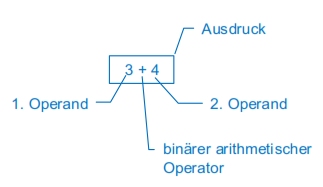
\includegraphics[width=0.6\textwidth]{pics/binaerer_Operator.png}	
	\end{minipage}
		
	\begin{minipage}[t]{9 cm}	
		\subsection{Postfix- und Präfixoperatoren}
			\subsubsection{Postfixoperatoren}
				Postfix-Operatoren sind unäre Operatoren, die nach (post) ihrem Operanden stehen.
				\vspace*{-0.2cm}
				\lstinputlisting[language=C,tabsize=2]{code/postfix.c}
				%\vspace*{0.1cm}
				$i$ wird auf den Bildschirm geschrieben, anschliessend inkrementiert.
	\end{minipage}
	\hspace*{1cm}		
	\begin{minipage}[t]{9 cm}
			\subsubsection{Präfixoperatoren}
				Präfix-Operatoren sind unäre Operatoren, die vor (prä) ihrem Operanden stehen.
				\vspace*{-0.2cm}
				\lstinputlisting[language=C,tabsize=2]{code/praefix.c}
				%\vspace*{0.1cm}
				$i$ wird zuerst inkrementiert, dann auf den Bildschirm geschrieben.
		\end{minipage}

		\begin{minipage}[t]{8 cm}	
			\subsection{Ausdrücke und Anweisungen \verweis{7.2}}
				\subsubsection{Ausdrücke}
					\begin{compactitem}
						\item hat immer einen Rückgabewert (Typ ist\\ durch Operanden bestimmt)
						\item kann Teil eines grösseren Ausdrucks sein
						\item kann eine Anweisung werden\\\\Beispiel: $3$ $(int)$ $+$ $4.5$ $(double)$
					\end{compactitem}
				\subsubsection{Anweisungen}
					\begin{compactitem}
						\item kann keinen Rückgabewert haben
						\item kann nicht Teil eines grösseren Ausdrucks sein
						\item Selektions-, Iterations-, Sprung-, Ausdrucksanweisung\\\\
						Beispiel: $while$ $(a\ \ \textgreater\ \ 14)$
					\end{compactitem}
		\end{minipage}
		\hspace*{1cm}
		\begin{minipage}[t]{9 cm}
			\subsection{Nebeneffekte \verweis{7.3}}
				\begin{compactitem}
					\item Bei Nebeneffekten wird nebst der eigentlichen Aufgabe noch eine weitere
					Operation in dieselbe Anweisung gepackt (häufig mit Präfix- und Postfix Operatoren)
					\item zurückhaltend einsetzen!!\\\\
					Beispiel:\\
					$j = i++;$
					\ \ \ \ ist äquivalent zu\\\\
					$j = i;$\\
					$i = i+1;$ \ \ \ \ \ \ $// j++$; 	
				\end{compactitem}
		\end{minipage}
		\subsection{Auswertungsreihenfolge \verweis{7.4}}
			\subsubsection{Regeln}
				\begin{enumerate}
					\item Wie in der Mathematik werden als erstes Teilausdrücke in Klammern ausgewertet.
					\item Dann werden Ausdrücke mit unären Operatoren ausgewertet. Unäre Operatoren werden von rechts nach links angewendet, d.h.
					\begin{enumerate}
						\item zuerst werden die Postfix-Operatoren auf ihre Operanden
						\item und dann die Präfix-Operatoren auf ihre Operanden angewendet.
					\end{enumerate}
					\item Abschliessend werden Teilausdrücke mit mehrstelligen Operatoren gemäss der Priorität der Operatoren ausgewertet.
					\item Bei gleicher Priorität der Operatoren entscheidet die Assoziativität (von links
					nach rechts oder von rechts nach links)
				\end{enumerate}
			\begin{minipage}[t]{9 cm}
				\subsubsection{Prioritätstabelle}
					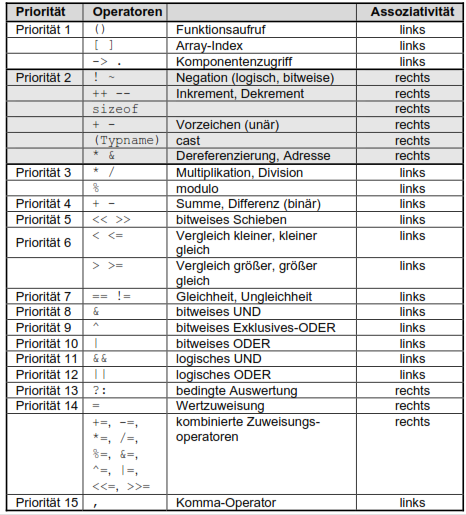
\includegraphics[width=1\textwidth]{pics/priotabelle.png}
			\end{minipage}
			\hspace*{0.5cm}
			\begin{minipage}[t]{8 cm}
				\subsubsection{Beispiele zur Auswertungsreihenfolge}
					\begin{enumerate}
						\item $*p++$\\\\
						Zuerst wird der Pointer p inkrementiert, der Rückgabewert von $p++$ ist $p$! Dieser 
						Rückgabewert (das noch nicht inkrementierte $p$) wird nun dereferenziert.
						\item $*++p$\\\\
						Zuerst wird der Pointer inkrementiert, der Rückgabewert von $++p$ ist der inkrementierte Pointer, dann wird (das inkrementierte) $p$ dereferenziert.
						\item $(*p)++$\\\\
						Zuerst wird der Pointer dereferenziert, anschliessend wird $*p$, d.h. der Inhalt der 
						Speicherzelle, auf welche $p$ zeigt, inkrementiert.
					\end{enumerate}
			\end{minipage}\\\\
			\begin{minipage}[t]{9 cm}
				\subsubsection{Assoziativität: links nach rechts oder rechts nach links?}
					\begin{compactitem}
						\item Ist meistens aufgrund der Operation intuitiv klar\\ (von links nach rechts ist häufiger)
						\item Achtung: Assoziativität legt die
						Reihenfolge der Operatoren fest, sie sagt
						aber nichts über die Reihenfolge der Auswertung der Operanden aus
					\end{compactitem}
					\hspace*{0.7cm}
					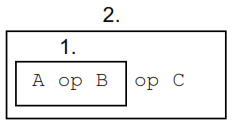
\includegraphics[width=0.3\textwidth]{pics/assoziativitaet.png}
					\begin{compactitem}
						\item Nebeneffekte sehr behutsam nützen!! 
					\end{compactitem}
			\end{minipage}
			\hspace*{0.5cm}
			\begin{minipage}[t]{8 cm}
				\subsubsection{Beispiel Pointer mit Post- /Prefix- Inkrement}
					\lstinputlisting[language=C,tabsize=2]{code/pointer_post-praefix_inkrement.c}
					\begin{tabular}{|l|r|r|}
					  \hline
					  Operation &  *p & p \\
					  \hline
					  Start & 4 & $0x22cca0$ \\
					  $*p++$ & 4 & $0x22cca4$ \\
					  $*++p$ & 66 & $0x22cca8$ \\
					  $*(p++$ & 66 & $0x22ccac$ \\
					  $(*p)++$ & 234 & $0x22ccac$ \\
					  $*pp$ & 235 & $0x22ccac$ \\
					  \hline
					\end{tabular}
			\end{minipage}\\\\
				\begin{minipage}[t]{13 cm}
				\subsection{L-Werte und R-Werte \verweis{7.5}}
					\begin{compactitem}
						\item Ausdrücke haben eine unterschiedliche Bedeutung, je nachdem, ob sie links oder rechts vom Zuweisungsoperator stehen.
						\item Ein Ausdruck stellt einen L-Wert (lvalue oder left value) dar, wenn er
						sich auf ein Speicherobjekt bezieht. Ein solcher Ausdruck kann links (und rechts) des Zuweisungsoperators stehen.
						\item Ein Ausdruck, der sich nicht auf ein Speicherobjekt bezieht, kann nur
						rechts des Zuweisungsoperators stehen. Er wird als R-Wert (rvalue oder right value) bezeichnet. Einem R-Wert kann nichts zugewiesen werden.\\
						\lstinputlisting[language=C,tabsize=2]{code/l-r-wert.c}
					\end{compactitem}
				\end{minipage}
				\hspace*{1cm}
				\begin{minipage}[t]{5 cm}
					\vspace*{-0.2cm}
					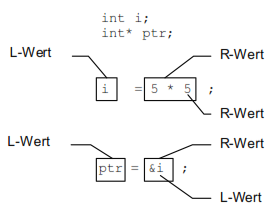
\includegraphics[width=1\textwidth]{pics/l-r-wert1.png}
					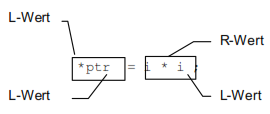
\includegraphics[width=1\textwidth]{pics/l-r-wert2.png}
				\end{minipage}\\
				\subsubsection{Zugriff auf L- und R-Werte}
					\begin{compactitem}
						\item Ein lvalue erfordert immer Schreibzugriff
						\item Auf einen rvalue wird nur lesend zugegriffen
						\item Es gibt auch nicht modifizierbare lvalues. Auf diese kann auch nur lesend zugegriffen werden.
					\end{compactitem}
			\subsection{Operatoren im einzelnen \verweis{7.6}}
				\begin{minipage}[t]{9 cm}
					\subsubsection{Unäre arithmetische Operatoren}
						\begin{compactitem}
							\item Positiver Vorzeichenoperator $+A$
							\item Negativer Vorzeichenoperator $-A$
							\item Postfix-Inkrementoperator $A++$
							\item Präfix-Inkrementoperator $++A$
							\item Postfix-Dekrementoperator $A- -$
							\item Präfix-Dekrementoperator $- -A$
						\end{compactitem}
				\end{minipage}
				\hspace*{0.5cm}
				\begin{minipage}[t]{9 cm}
					\subsubsection{Binäre arithmetische Operatoren}
						\begin{compactitem}
							\item Additionsoperator $A + B$
							\item Subtraktionsoperator $A - B$
							\item Multiplikationsoperator $A * B$
							\item Divisionsoperator $A / B$
							\item Modulooperator $A \% B$   
						\end{compactitem}	
				\end{minipage}\\\\
				\begin{minipage}[t]{9 cm}
					\subsubsection{Zuweisungsoperatoren}
						\begin{compactitem}
							\item Zuweisungsoperator $A = B$
							\item Kombinierte Zuweisungsoperatoren
							\begin{compactitem}
								\item Alle arithmetischen und logischen Operatoren haben zusammen mit dem
								Zuweisungsoperator eine verkürzte Form, die das Schreiben verkürzt (mehr
								nicht)
								\item Beispiel:\\
								$a = a / b;$\\
								kann verkürzt geschrieben werden als\\
								$a /= b;$
							\end{compactitem}
						\end{compactitem}
				\end{minipage}
				\hspace*{0.5cm}
				\begin{minipage}[t]{6 cm}
					\subsubsection{Relationale Operatoren  (Vergleichsoperatoren)}
						\begin{compactitem}
							\item Gleichheitsoperator $A == B$
							\item Ungleichheitsoperator $A != B$
							\item Grösseroperator $A \textgreater \ \ B$
							\item Kleineroperator $A \textless \ \ B$
							\item Grössergleichoperator $A \textgreater= B$
							\item Kleinergleichoperator $A \textless= B$ 
						\end{compactitem}	
				\end{minipage}\\\\
				\begin{minipage}[t]{9 cm}
					\subsubsection{Logische Operatoren}
						\begin{compactitem}
							\item Logisch UND (AND) $A \&\& B$
							\item Logisch ODER (OR) $A || B$
							\item Logisch NICHT (NOT) $!A$\\\\
							0 = false, falsch\\
							1 = true, wahr (genauer: ungleich 0)
						\end{compactitem}
				\end{minipage}
				\hspace*{0.5cm}
				\begin{minipage}[t]{9 cm}
					\subsubsection{Bit-Operatoren}
						\begin{compactitem}
							\item Bitweises AND $A \& B$
							\item Bitweises OR $A | B$
							\item Bitweises NOT (Inverter) $\textasciitilde A$
							\item Bitweises XOR $A \wedge B$ 
						\end{compactitem}	
				\end{minipage}
				
				\subsubsection{Schiebe- (Shift-) Operatoren}
					\begin{compactitem}
						\item Rechts-Shift um n Bits $A \textgreater \ \textgreater \ \ n$
						\item Links-Shift um n Bits $A \textless \  \textless \ \ n$
					\end{compactitem}
										
				\begin{minipage}[t]{9 cm}
					\subsubsection{Bedingungsoperator (Ternärer Operator)}
						$A ? B : C$\\\\
						Ist eine verkürzte Schreibweise für
						\lstinputlisting[language=C,tabsize=2]{code/Ternaerer_Operator.c}
				\end{minipage}
				\hspace*{0.5cm}
				\begin{minipage}[t]{9 cm}
					
						\vspace*{0.5cm}
						Beispiel Maximum von zwei Zahlen a, b ermitteln:
						\lstinputlisting[language=C,tabsize=2]{code/Ternaerer_Operator2.c}
						entspricht:
						\lstinputlisting[language=C,tabsize=2]{code/Ternaerer_Operator3.c}	
				\end{minipage}
			\subsection{Type Cast (Typumwandlungsoperator) \verweis{7.7}}	
				\begin{minipage}[t]{9 cm}
					\subsubsection{Implizite Typumwandlung}
						Bei der impliziten Typumwandlung wird Umwandlung nicht im Code aufgeführt. Sie wird vom Compiler automatisch anhand der Datentypen von Variablen bzw. Ausdrücken erkannt und durchgeführt.\\\\
						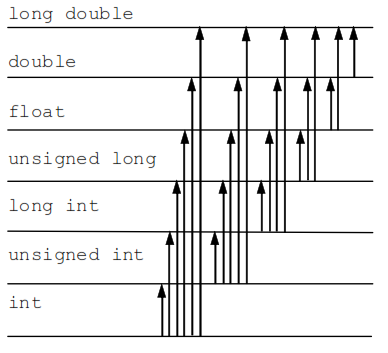
\includegraphics[width=0.5\textwidth]{pics/typecast.png}	
						\\\\Beispiel:
						\vspace*{-0.2cm}
						\lstinputlisting[language=C,tabsize=2]{code/Implizite_Typumwandlung.c}	
				\end{minipage}
				\hspace*{0.5cm}
				\begin{minipage}[t]{9 cm}
					\subsubsection{Explizite Typumwandlung}
						\begin{compactitem}
							\item Nebst den impliziten (automatischen) Typumwandlungen kann mit Hilfe des
							cast-Operators eine explizite Typumwandlung bewirkt werden.
							\item Der Programmierer ist verantwortlich, dass die Umwandlung keine Probleme
							ergibt.
							(z.B. Umwandlung von grosser Zahl in kleineren Typ)
							\item Syntax:
							(Zieltyp)Ausdruck
							\\\\Beispiel:
							\lstinputlisting[language=C,tabsize=2]{code/Implizite_Typumwandlung2.c}
						\end{compactitem}
					\subsubsection{Erlaubte Typenumwandlung}
						\begin{compactitem}
							\item Zwischen skalaren Typen (Integer, Floating Points, Pointer)
							\item Von skalarem Typ in $void$
						\end{compactitem}
				\end{minipage}
			\subsection{Gültigkeitsbereiche von Namen (Scope)}				
				\begin{compactitem}
					\item Compiler arbeitet dateiweise
					\item Namen in einer anderen Datei sind dem Compiler nicht bekannt
					\item (Globale) Variablen, welche in einer anderen Datei definiert werden, können 
					mit Hilfe des extern-Statements bekannt gemacht werden
					\item Durch das extern-Statement wird kein Speicherplatz reserviert.\\
					$extern$ $int$ $Foo\_globalVariable$;
					\item Funktionsprototypen und Definitionen, die von anderen Modulen genutzt
					werden können (Schnittstellen), werden in einer Headerdatei definiert
					\item Durch $\#include$ der Headerdatei wird der Header geladen und die Namen somit bekannt gemacht.
				\end{compactitem}